%%
%% 研究報告用スイッチ
%% [techrep]
%%
%% 欧文表記無しのスイッチ(etitle,jkeyword,eabstract,ekeywordは任意)
%% [noauthor]
%%

\documentclass[submit,techreq,noauthor,onecolumn]{ipsj}


\usepackage[dvipdfmx]{graphicx}
\usepackage{latexsym}

\def\Underline{\setbox0\hbox\bgroup\let\\\endUnderline}
\def\endUnderline{\vphantom{y}\egroup\smash{\underline{\box0}}\\}
\def\|{\verb|}

\setcounter{page}{1}

\pagestyle{empty}
\begin{document}


\title{Applied Type System \\ {\huge\it (Extended Abstract)}}

\author{Hongwei Xi - Boston University}{}{}

\begin{abstract}
Pure Type Systemフレームワーク ({\it PTS}) は型システムをデザイン/形式化する単純で一般的なアプローチを提供します。
けれども依存型の存在を認めると、一般帰納、再帰型、作用 (例: 例外、参照、入出力)、などのような実際のプログラミング機能の多くに {\it PTS} を適用させることが難しくなります。
この論文では、実際のプログラミング機能をサポートする型システムをたやすくデザイン/形式化できる、新しい Applied Type System ({\it ATS}) フレームワークを提案します。
{\it ATS} の鍵となる突出した機能は、コンストラクトされて評価されるプログラムを含む動的な部分から、形作られて根拠となる型を含む静的な部分を完全に分離することにあります。
この分離を用いると、プログラムが型の中に現われることは不可能になります。({\it PTS} では許可されていました。)
{\it ATS} の形式的な開発だけでなく、実用的なプログラミングのための型システムを作るフレームワークとして {\it ATS} を使った例もいくつか紹介します。

\vspace{2mm}

この翻訳の元論文は http://www.ats-lang.org/PAPER/ATS-types03.pdf で、Japan ATS User Group http://jats-ug.metasepi.org/ によって翻訳されています。
また、この論文はフルペーパーである http://www.cs.bu.edu/$\sim$hwxi/academic/drafts/ATS.pdf の要約です。
\end{abstract}

\maketitle
\thispagestyle{empty}

\section{はじめに}

Pure Type Systemフレームワーク ({\it PTS}) [Bar92] は型システムをデザイン/形式化する単純で一般的なアプローチを提供します。
けれども依存型の存在を認めると、実際のプログラミング機能の多くに {\it PTS} を適用させることが難しくなります。
とりわけ、一般帰納 [CS87]、再帰型 [Men87]、作用 [HMST95]、例外 [HN88]、入出力が存在するとき {\it PTS} を使って純粋性を担保するためには、多大な努力が必要になることを私達は学びました。
このような {\it PTS} の限界に対処するために、実際のプログラミング機能をサポートする型システムをたやすくデザイン/形式化できる、新しい Applied Type System ({\it ATS}) フレームワークを提案します。
{\it ATS} の鍵となる突出した機能は、コンストラクトされて評価されるプログラムを含む動的な部分から、形作られて根拠となる型を含む静的な部分を完全に分離することにあります。
この分離は Dependent ML (DML) [XP99,Xi98] で開発された制限付きの依存型の成果に由来していて、参照や例外のような作用の存在下でも依存型を柔軟にサポートします。
また、{\it ガード型} ({\it guarded types}) と {\it アサート型} ({\it asserting types}) という2つの新しく馴染みのない型を導入することで、{\it ATS} では {\it PTS} よりも柔軟に効果的にプログラムの不変条件を捕捉することができることを示します。

{\it ATS} のデザインと形式化がこの論文の主な主張であり、[Zen97,XP99,XCC03] と似たアイデアを使った研究成果です。
{\it ATS} を使うと、{\it PTS} の生来の欠陥を乗り越えて、依存型の存在下で多くの一般的なプログラミング機能をサポートする型システムをたやすく設計できます。
私達は現在 {\it ATS} に基づいた型システムを持ち、(DML で開発されたような) 依存型のみではなく guarded recursive datatypes [XCC03] をもサポートする、型付き関数型プログラミング言語を設計/実装している最中です。
Scheme が導入したようなアプローチ、つまり既存の言語に新しい言語構造を実装するような手法で、{\it ATS} を用いて多様な言語拡張をサポートできないか私達は探求しています。
とりわけ、オブジェクト指向プログラミング [XCC03]、メタプログラミング [XCC03,CX03]、型クラス [XCC02] のようないくつかのプログラミング機能をこの手法で扱えることを、私達は既に示しています。

この論文の残りは次のような構成になっています。
2章では、{\it ATS} フレームワークの詳細な開発成果を示します。
{\it ATS} で構成された汎用的な Applied Type System である ATS を形式化し、それからsubject reductionとprogress定理を定義します。
3章では、一般帰納、パターンマッチ、作用のような一般的で現実的なプログラミング機能のいくつかに、{\it ATS} を拡張して順応させます。
4章では、applied type system の興味深い例をいくつか示します。
最後に、関連研究と開発の将来の可能性について紹介した後、結論を述べます。
この論文はオンライン [Xi03] から入手できます。

\begin{figure}[h]
\centering
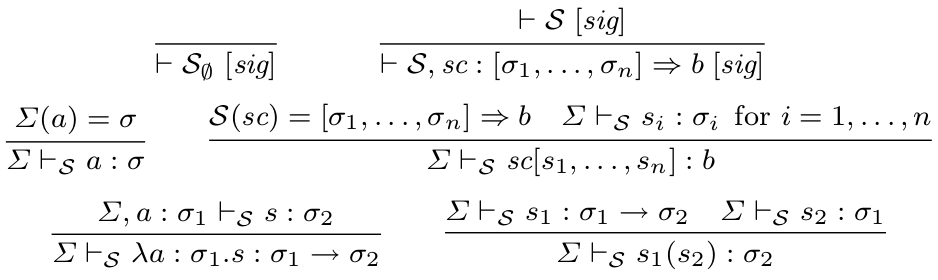
\includegraphics[width=11cm]{img/fig1_rules.png}
\caption{staticsを表わすシグニチャフォーマット規則と分類規則}
\label{fig:fig1_rules}
\end{figure}

\section{Applied Type System}

この章では Applied Type System ({\it ATS}) フレームワークの形式化を示します。
ここでは {\it ATS} で形式化された型システムを表わすのに {\it applied type system} という用語を使います。
この後の説明では、静的な要素 (statics) と動的な要素 (dynamics) から成る一般的な applied type system として、ATS を定義します。
直感的に、statics と dynamics はそれぞれ型とプログラムを扱っています。
単純化のために、statics は簡単な純粋型付き言語であると仮定します。
そしてこの言語の型を {\it 種} ({\it sort}) という名前で呼ぶことにします。
statics の項を {\it 静的な項} ({\it static term}) と呼びます。
また dynamics の項を {\it 動的な項} ({\it dynamic term}) と呼びます。
そして、特別な種 {\it type} の静的な項は dynamics の型として機能します。


\subsection{Statics}

静的な要素の形式的な表現を示します。
基礎種を {\it b} と表わします。
2つの特別な基礎種 {\it type} と {\it bool} が存在すると仮定します。

\begin{figure}[h]
\centering
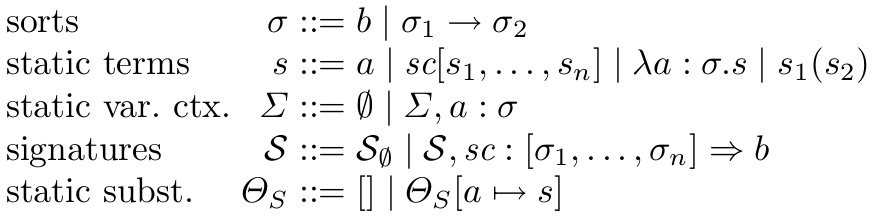
\includegraphics[width=9cm]{img/infig21_formaldesc.png}
\end{figure}

\noindent 静的な項の変数は $a$ を使って表わし、静的な項の集合を $s$ で表わします。
静的な定数 {\it sc} を宣言することもできます。
この定数は、静的な定数コンストラクタ {\it scc} もしくは静的な関数定数 {\it scf} のどちらかです。
sc種 (sc-sorts) を表わすのに [$\sigma_1$, $\ldots$ ,$\sigma_n$] $\Rightarrow$ {\it b} を使い、これは静的な定数に割り当てられます。
静的な定数 {\it sc} が与えられたとき、もし なんらかの種 $\sigma_1$, $\ldots$ ,$\sigma_n$ について {\it sc} にsc種 [$\sigma_1$, $\ldots$ ,$\sigma_n$] $\Rightarrow$ {\it b} が割り当てられていて、$i = 1, \ldots ,n$ について $s_i$ に種 $\sigma_i$ を割り当てることができるなら、種 {\it b} の項 {\it sc}[$s_1$, $\ldots$ ,$s_n$] を作ることができます。
誤解を生じない場合は、{\it sc}[] を {\it sc} と書くことができます。
sc種は (標準の) 種とは見なされないことに注意してください。

静的な変数を静的な項に写像するような静的な置換を $\Theta_S$ で表わします。
また $\Theta_S$ のドメインを {\bf dom}($\Theta_S$) で表わします。
空の写像を表わすのに [] と書きます。
{\it a} $\notin$ {\bf dom}($\Theta_S$) を仮定したとき、{\it a} から {\it s} へのリンクで $\Theta_S$ を拡張した写像を $\Theta_S$[$a \mapsto s$] と表わします。
また、$\Theta_S$ を構文 $\bullet$ に適用した結果を表わすのに、$\bullet[\Theta_S]$ と書きます。
構文 $\bullet$ は、静的な項、静的な項の列、この後で定義する動的な可変コンテキスト、のいずれかを表わします。

シグニチャは宣言された静的な定数 $sc$ に割り当てたsc種を表わし、そのシグニチャの形成ルールは図\ref{fig:fig1_rules}で与えられます。
初期シグニチャ $S_0$ が次の宣言を含むことを仮定しています。

\begin{figure}[h]
\centering
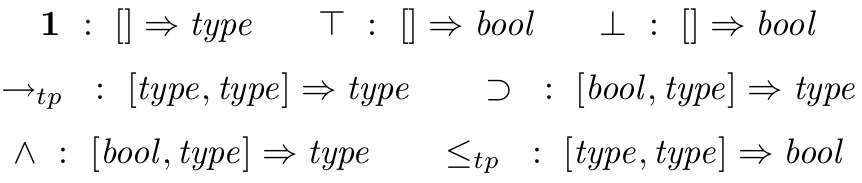
\includegraphics[width=9cm]{img/infig21_initialsig.png}
\end{figure}

\noindent これらは、'':'' の左側は静的な定数で、その右側には一致するsc種が割り当てられています。
また、それぞれの種 $\sigma$ について、$S_0$ は2つの静的コンストラクタ $\forall_\sigma$ と $\exists_\sigma$ にsc種 [$\sigma \rightarrow_{tp} type$] $\Rightarrow$ {\it type} を割り当てることを仮定しています。
静的な定数を表わすのに中置表記を使うこともできます。
例えば、$\rightarrow_{tp} [s_1,s_2]$ を表わすのに $s_1 \rightarrow_{tp} s_2$ のように、$\leq_{tp} [s_1,s_2]$ を表わすのに $s_1 \leq_{tp} s_2$ のように書けます。
さらに、$\forall_a [\lambda a : \sigma.s]$ と $\exists_a [\lambda a : \sigma.s]$ をそれぞれ $\forall_a : \sigma.s$ と $\exists_a : \sigma.s$ のように書くこともできます。
staticsの分類規則は図\ref{fig:fig1_rules}で与えられますが、大部分は標準的なものです。
例えば、$\emptyset \vdash_{S_0} \forall_{type} [\lambda a : type.a \rightarrow_{tp} a] : type$ が導けるので、$\forall a : type.a \rightarrow_{tp} a$ は種typeを割り当てることができる静的な項です。
なんらかの種 $\sigma_1$, $\ldots$ ,$\sigma_n$ についてsc種 [$\sigma_1$, $\ldots$ ,$\sigma_n$] $\Rightarrow$ {\it type} を割り当てられるなら、静的なコンストラクタ$sc$は型コンストラクタです。
例えば {\bf 1}, $\rightarrow_{tp}$, $\supset$, $\wedge$, $\forall_\sigma$, $\exists_\sigma$ は全て型コンストラクタですが、$\leq_{tp}$ は型コンストラクタではありません。
直感的には、{\bf 1} は通常のユニット型を表わし、$\rightarrow_{tp}$ は関数型を作り、$\leq_{tp}$ は型におけるサブタイピング関係を表わします。
静的なコンストラクタ $\supset$ と $\wedge$ はそれぞれガード型 (guarded types) とアサート型 (asserting types) を作り、これらは後で解説します。

静的な変数群に種を割り当てるような、静的な可変コンテキストを表わすのに $\Sigma$ を使います;
{\bf dom}($\Sigma$) は $\Sigma$ で宣言された静的な変数の組です;
もし $a : \sigma$ が $\Sigma$ で宣言されていたら、$\Sigma (a) = \sigma$ です。
例によって、$\Sigma$ において静的な変数 $a$ は一回しか宣言できません。
もし $\Sigma \vdash s : bool$ が導けるなら、静的な項 $s$ は $\Sigma$ の下の {\it 命題} ({\it proposition}) と呼ばれます。
(なんらかの静的な可変コンテキストの下で) 命題を表わすのに $P$ を使います。
$P \supset s$ という形の型を表わすのに {\it ガード型} ({\it guarded type})、$P \wedge s$ という形の型を表わすのに {\it アサート型} ({\it asserting type}) という名前を使います。
これらは両方とも次の例で使います。

\noindent {\it Example 1.}
$int$ を整数
\footnote{形式的には、それぞれの整数 $n$ について、sc種 $[] \Rightarrow int$ の静的なコンストラクタ $\underline n$ が存在し、$\underline n$[] は $n$ に相当する種 $int$ の静的な項であることを言う必要があります。
}
を表わす種に、{\bf list} をsc種 $[type,int] \Rightarrow type$ の型コンストラクタとすると、次の静的な項は型になります:

\begin{figure}[h]
\centering
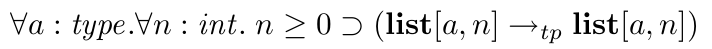
\includegraphics[width=9cm]{img/infig21_example1_list1.png}
\end{figure}

\noindent 直感的には、もし {\bf list}[$s$,$n$] がそれぞれの要素の型が $s$ で長さ $n$ のリストを表わす型だとすると、リストの長さを変えないようなリストからリストへの関数を、上記の型は意図していると言えます。
また次の型は、もし与えられたリストが空でなければそのリストのtailを返し、そうでなければ単に例外を発生させるような関数に割り当てることを意図しています。

\begin{figure}[h]
\centering
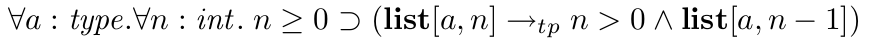
\includegraphics[width=11cm]{img/infig21_example1_list2.png}
\end{figure}

アサート型 $n > 0$ $\wedge$ {\bf list}[$a$, $n-1$] は、長さ $n$ のリストにこの関数を適用した後、もしこの関数が返るなら、 $n > 0$ であり返値が長さ $n-1$ のリストであるという不変条件を捕捉しています。
これはいくぶん興味深い機能で、後のExample 2で詳しく解説します。
Dependent ML [XP99,Xi98] における研究でも既にアサート型がありましたが、
アサート型の正確な概念はこれまで形式化されたことがありませんでした:
DMLではこの論文でアサート型と呼んでいるものをシミュレートするのにサブセット種を使わねばなりませんでした。

{\it PTS} でのデザインと同様に、{\it ATS} でのデザインにおいても型の等価性は難解な問題です。
けれどもさらなる研究によって、{\it ATS} における型の等価性はサブタイピング関係 $\leq_{tp}$ によって定義できることが明らかになりました。
2つの型 $s_1$ と $s_2$ が与えられたとき、もし命題 $s_1 \leq_{tp} s_2$ と命題 $s_2 \leq_{tp} s_1$ の両方が成立するなら、$s_1$ と $s_2$ は等しいと言えるのです。
一般に、(ある前提の元に) 与えられた命題が成立するかどうか決定する必要があります。
そこで、次ような制約関係の概念を導入します。

\begin{figure}[h]
\centering
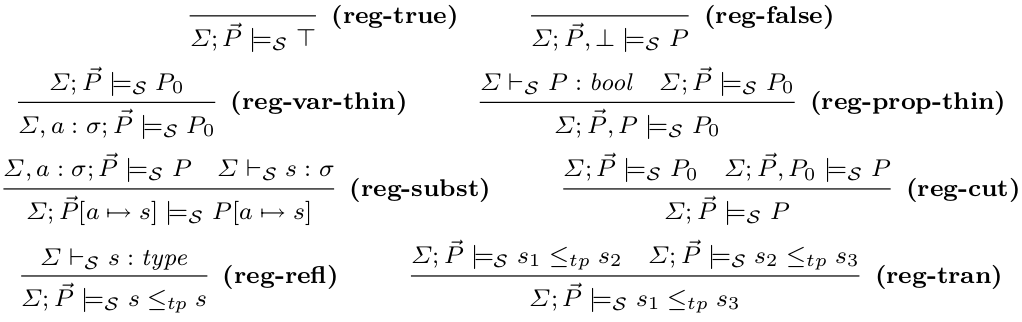
\includegraphics[width=14cm]{img/fig2_regularity_rules.png}
\caption{規則ルール}
\label{fig:fig2_regularity_rules}
\end{figure}

{\bf Definition 1.}
$S$, $\Sigma$, $\vec{P}$, $P_0$ をそれぞれ 静的なシグニチャ, 静的な可変コンテキスト, $\Sigma$ の下での命題の組, $\Sigma$ の下での1つの命題であるとします。
もし次の規則条件が満たされるなら、関係 $\Sigma$; $\vec{P} \models_S P_0$ は正規の制約関係であると言います:

\begin{enumerate}
  \item 図\ref{fig:fig2_regularity_rules} の規則ルール全てが有効である; すなわちそれぞれの規則ルールについて、もしルールの根拠が成立するならルールの結論が成立し、なおかつ
  \item $\Sigma; \vec{P} \models_S s_1 \rightarrow_{tp} s_2 \leq_{tp} s'_1 \rightarrow_{tp} s'_2$ は $\Sigma; \vec{P} \models_S s'_1 \leq_{tp} s_1$ と $\Sigma; \vec{P} \models_S s_2 \leq_{tp} s'_2$ を意味し、なおかつ
  \item $\Sigma; \vec{P} \models_S P \supset s \leq_{tp} P' \supset s'$ は $\Sigma; \vec{P},P' \models_S P$ と $\Sigma; \vec{P},P' \models_S s \leq_{tp} s'$ を意味し、なおかつ
  \item $\Sigma; \vec{P} \models_S P \wedge s \leq_{tp} P' \wedge s'$ は $\Sigma; \vec{P},P \models_S P'$ と $\Sigma; \vec{P},P \models_S s \leq_{tp} s'$ を意味し、なおかつ
  \item $\Sigma; \vec{P} \models_S \forall a : \sigma.s \leq_{tp} \forall a : \sigma.s'$ は $\Sigma , a: \sigma; \vec{P} \models_S s \leq_{tp} s'$ を意味し、なおかつ
  \item $\Sigma; \vec{P} \models_S \exists a : \sigma.s \leq_{tp} \exists a : \sigma.s'$ は $\Sigma , a: \sigma; \vec{P} \models_S s \leq_{tp} s'$ を意味し、なおかつ
  \item $\emptyset; \emptyset \models_S scc[s_1,\ldots,s_n] \leq_{tp} scc'[s'_1,\ldots,s'_{n'}]$ は $scc = scc'$ を意味します
\end{enumerate}

\noindent $\Sigma; \vec{P} \models_S P_0$ と書くときはいつでも $P \in \vec{P},P_0$ について $\Sigma \vdash_S P : bool$ を導出できることを仮定していることに注意してください。

\noindent ATSのdynamicsを作るとき、制約関係を必要とします。全ての単一の規則条件と同様に、全ての単一の規則ルールはsubject reduction定理(Theorem 1)とprogress定理(Theorem 2)を規定するために後で使うことになります。
一般に、{\it ATS} フレームワークは制約関係の上にパラメータ化されています。
この時点では、制約関係の決定可能性を気にする必要はありません。
それぞれの制約関係 $\models_S$ について、どのような $\Sigma, \vec{P}$ と $P_0$ が与えられても $\Sigma; \vec{P} \models_S P_0$ が満たされるかどうか、決定してくれるオラクルが存在することを単純に仮定することができます。
後で、制約関係を決定する実用的なアルゴリズムを持つapplied type systemの例をいくつか紹介します。

非叙述性 (impredicativity) のために、与えられたシグニチャ $S$ について制約関係 $\models_S$ をいかに厳密に定義できるかは、一般にかなり難しい問題です。
[Xi03] では、モデル理論的なアプローチで私達はこの問題を解決しています。


\subsection{Dynamics}

ATS の dynamics は型付き言語で、種 {\it type} の静的な項は dynamics における型です。
動的な定数をいくつか宣言することができ、引数 $n$ の動的な定数 $dc$ それぞれに次の形の dc 型を割り当てることができます。

\begin{figure}[h]
\centering
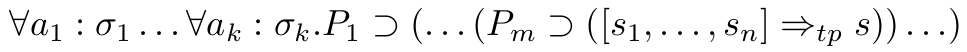
\includegraphics[width=10cm]{img/infig22_dc-type.png}
\end{figure}

\noindent このとき $s_1,\ldots,s_n,s$ は型であると仮定しています。
$dc$ が動的なコンストラクタ $dcc$ である場合、なんらかの型コンストラクタ $scc$ について 型 $s$ は $scc[\vec{s}]$ の形を取れなければなりません。
すると $dcc$ は $scc$ と関連があると言えるのです。
静的な項の (空である可能性のある) 列を表わすのに $\vec{s}$ を使っていることに注意してください。
例えば、次のようにdc型を割り当てることで、2つの動的なコンストラクタ {\it \underline{nil}} と {\it \underline{cons}} を型コンストラクタ {\bf list} と関連付けることができます。

\begin{figure}[h]
\centering
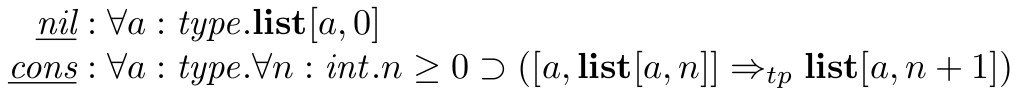
\includegraphics[width=10cm]{img/infig22_nil_cons.png}
\end{figure}

\noindent このとき、要素の型が $a$ で長さが $n$ のリストを表わす型として {\bf list}$[a,n]$ を使っています。

動的な値を動的な項に写像する動的な置換を $\Theta_D$ で表わします。
また $\Theta_D$ のドメインを {\bf dom}($\Theta_D$) で表わします。
静的な置換と同じように、動的な置換を形成して適用するような構文を示すことを省きます。
{\bf dom}($\Theta^1_D$) $\cap$ {\bf dom}($\Theta^2_D$) $= \emptyset$ となるような $\Theta^1_D$ と $\Theta^2_D$ が与えられたとき、$\Theta^1_D$ と $\Theta^2_D$ の和集合を $\Theta^1_D \cup \Theta^2_D$ で表わします。

任意の構文を $\bullet$ で表わすと、$\Sigma = a_1 : \sigma_1,\ldots,a_k : \sigma_k$ において、$\forall a_1:\sigma_1 \ldots \forall a_k:\sigma_k .\bullet$ を $\forall\Sigma.\bullet$ と書くことができます。
同様に、$\vec{P} = P_1,\ldots,P_m$ において $P_1 \supset (\ldots(P_m \supset \bullet)\ldots)$ を $\vec{P} \supset \bullet$ と書くことができます。
例えば、dc型は常に $\forall \Sigma.\vec{P} \supset ([s_1,\ldots,s_n] \Rightarrow_{tp} s)$ の形になります。
動的な定数の宣言を許可するために、シグニチャの定義を次のように拡張する必要があります。

\clearpage

\begin{figure}[h]
\centering
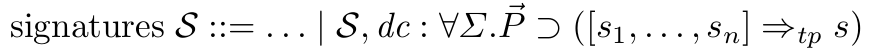
\includegraphics[width=9cm]{img/infig22_dynamic_sig.png}
\end{figure}

\noindent さらに、シグニチャを作るために次のような追加のルールが必要になります。

\begin{figure}[h]
\centering
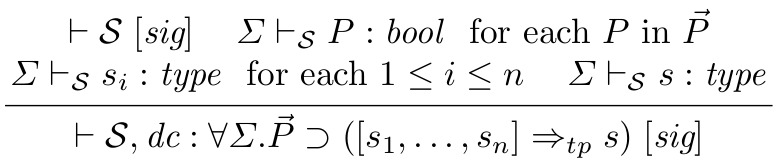
\includegraphics[width=9cm]{img/infig22_addtional_rule.png}
\end{figure}

\noindent 動的な項の変数として $x$ を、動的な項として $d$ を用いるとき、dynamicsの構文を図\ref{fig:fig3_syntax_dynamics} に示します。
引数の個数が $n$ の動的な定数 $dc$ が与えられたとき、引数 $d_1,\ldots,d_n$ への $dc$ の適用を $dc[d_1,\ldots,d_n]$ と書きます。
$n = 0$ の場合には $dc[]$ の代わりに $dc$ と書くこともできます。

\begin{figure}[h]
\centering
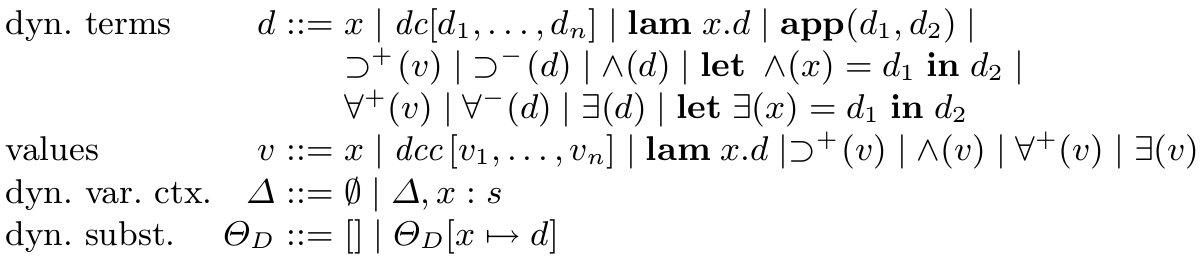
\includegraphics[width=14cm]{img/fig3_syntax_dynamics.png}
\caption{dynamicsの構文}
\label{fig:fig3_syntax_dynamics}
\end{figure}

\begin{figure}[h]
\centering
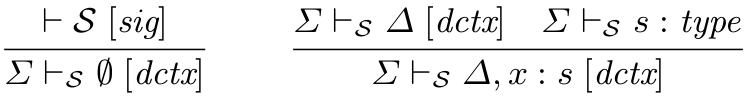
\includegraphics[width=8cm]{img/fig4_rules_dynamics.png}
\caption{動的な可変コンテキストを表わす形成ルール}
\label{fig:fig4_rules_dynamics}
\end{figure}

型の導出において帰納的な意味付けに必要なLemma 3を証明するために、標識 $\supset^+(\cdot)$, $\supset^-(\cdot)$, $\wedge(\cdot)$, $\forall^+(\cdot)$, $\forall^-(\cdot)$, $\exists(\cdot)$ を導入します。
これらの標識がないと、型の導出において帰納的証明を行なうことが、著しく困難になります。
Lemma 3を証明することも困難になってしまうでしょう。

$\Sigma \vdash_S \Delta [dctx]$ の形の判定は、$\Sigma$ と $S$ の下で $\Delta$ が well-formed な動的な可変コンテキストであることを示しています。
このような判定を導出するルールを図\ref{fig:fig4_rules_dynamics}に示します。
型付けされたコンテキトを $\Sigma; \vec{P}; \Delta$ で表わします。
次のルールは $\vdash_S \Sigma; \vec{P}; \Delta$ の形の判定を導出しています。

\begin{figure}[h]
\centering
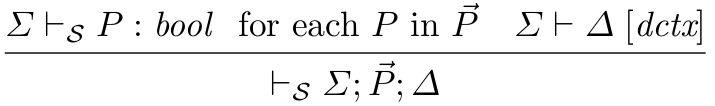
\includegraphics[width=7cm]{img/infig22_rule_deriving.png}
\end{figure}

\noindent これは $\Sigma; \vec{P}; \Delta$ が well-formed であることを示しています。

$\Sigma; \vec{P}; \Delta$ が well-formed な型付けされたコンテキストで、かつ $\Sigma \vdash_S s:type$ 導出できると仮定したとき、型付け判定は $\Sigma; \vec{P}; \Delta \vdash_S d:s$ の形を取ります。
制約関係 $\models_S$ が正則であると仮定したとき、このような判定を導くための型付けルールを図\ref{fig:fig5_typingrules_dynamics}に示します。
$\Sigma \vdash_S \Theta_S : \Sigma_0$ と書くとき、それぞれの $a \in {\bf dom}(\Theta_S) = {\bf dom}(\Sigma)$ について $\Sigma \vdash_S \Theta_S(a) : \Sigma(a)$ が導出できることを意味します。
型付けルールに関連する明らかな条件のいくつかを省略していることに注意してください。
例えば、ルール {\bf(ty-$\forall$-intro)} を適用するとき、$\vec{P}$, $\Delta$ もしくは $s$ において値 $a$ は自由に出現 (free occurrences) できません。
また値の形に、型付けルール {\bf (ty-gua-intro)} と {\bf (ty-$\forall$-intro)} の制約を付けています。
これは後でATSに作用を導入するための準備です。
\footnote{実際にはTheorem 2を成立させるために、型付けルール {\bf (ty-gua-intro)} の値に対する制約は、この時点でも必要です。}
技術的な理由で、ルール {\bf (ty-var)} を次のようなルールで置き換えます。

\clearpage

\begin{figure}[h]
\centering
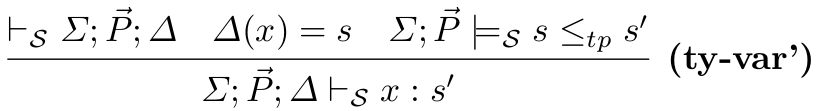
\includegraphics[width=8cm]{img/infig22_ty-var.png}
\end{figure}

\noindent これは {\bf (ty-var)} と {\bf (ty-sub)} を結合しています。
この置換は Lemma 2 成立させるために必要です。

\begin{figure}[h]
\centering
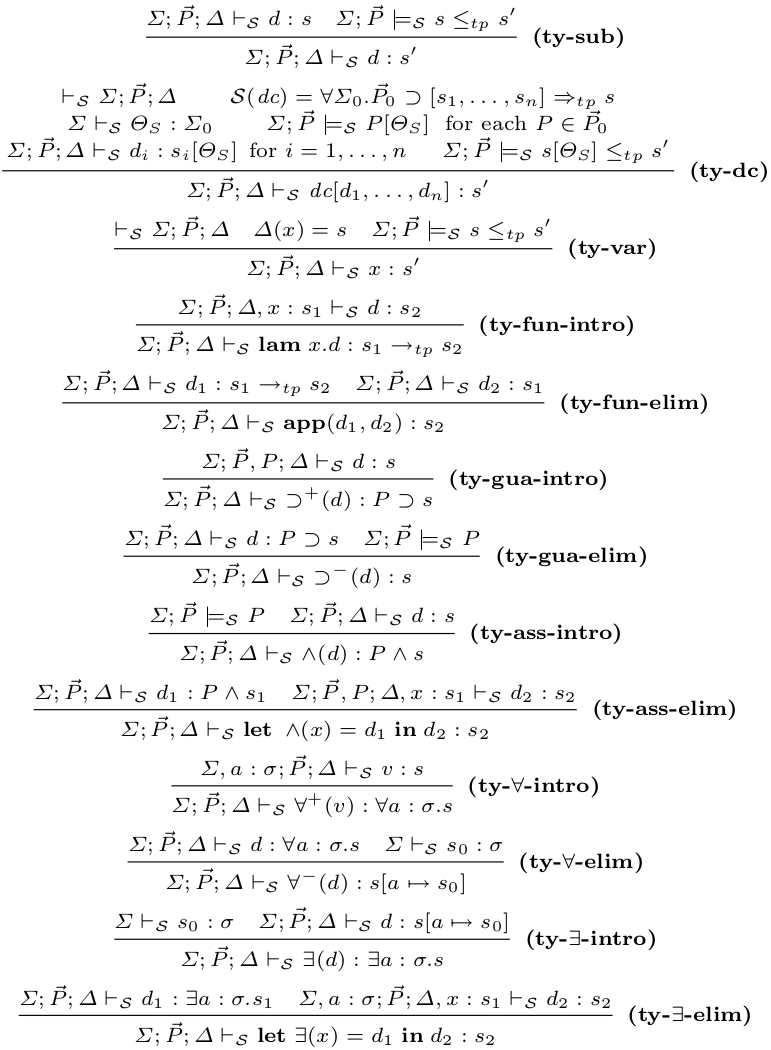
\includegraphics[width=12cm]{img/fig5_typingrules_dynamics.png}
\caption{dynamicsの型付けルール}
\label{fig:fig5_typingrules_dynamics}
\end{figure}

ここで、動的な項を評価するルールの表現に進む前に、ガード型とアサート型がセキュリティを強制する役割を演じるような、興味深いシナリオをスケッチしてみましょう。
これらの型を理解をさらに容易にしてくれるはずです。

\noindent {\it Example 2.}
\underline{$Secret$}は命題定数で、\underline{$password$}と\underline{$action$}が次のようなdc型が割り当てられた2つの関数で宣言されている、と仮定します。

\begin{figure}[h]
\centering
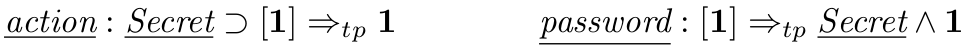
\includegraphics[width=10cm]{img/infig22_example2.png}
\end{figure}

\noindent \underline{$password$} を呼び出しが返る前になんらかのsecret情報を検証しなければならない、というような方法で関数 \underline{$password$} を実装することができます。
一方では、関数呼び出し \underline{$action$}$[\langle\rangle]$ をする前に、命題 \underline{$Secret$} を成立させなければなりません。
このとき、$\langle\rangle$ はユニット型 {\bf 1} の値を意味します。
もう一方、関数呼び出し \underline{$password$}$[\langle\rangle]$ が返った後では、命題 \underline{$Secret$} は成立しています。
従って、\underline{$action$} 呼び出しは次のプログラムパターンを意味していることになります:

\begin{figure}[h]
\centering
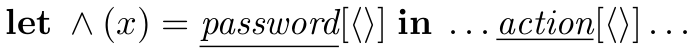
\includegraphics[width=7cm]{img/infig22_letin.png}
\end{figure}

\noindent 特に $x$ のスコープ外における \underline{$action$} 呼び出しは ill-typed です。
なぜなら命題 \underline{$Secret$} を成立させることができないからです。

値渡し (call-by-value) の動的な構文を動的な項に割り当てるために、次に定義する評価コンテキストを利用します:

\begin{figure}[h]
\centering
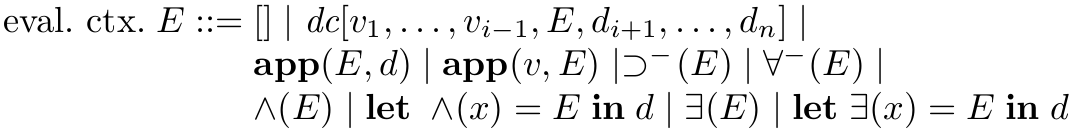
\includegraphics[width=11cm]{img/infig22_eval.png}
\end{figure}

\noindent {\bf Definition 2.}
簡約基 (redex) と簡約 (reducation) を次のように定義します。

\begin{itemize}
  \item ${\bf app}({\bf lam} x.d, v)$ は簡約基で、その簡約は $d[x \mapsto v]$ です。
  \item $\supset^- (\supset^+ (v))$ は簡約基で、その簡約は $v$ です。
  \item ${\bf let} \wedge (x) = \wedge (v) {\bf in} d$ は簡約基で、その簡約は $d[x \mapsto v]$ です。
  \item $\forall^- (\forall^+ (v))$ は簡約基で、その簡約は $v$ です。
  \item ${\bf let} \exists (x) = \exists (v) {\bf in} d$ は簡約基で、その簡約は $d[x \mapsto v]$ です。
  \item なんらかの値 $v$ に等しく定義された $dcf[v_1,\ldots,v_n]$ は簡約基で、その簡約は $v$ です。
\end{itemize}

\noindent なんらかの簡約基 $d$ とその簡約 $d'$ について $d_1 = E[d]$ かつ $d_2 = E[d']$ のような2つの動的な項 $d_1$ と $d_2$ が与えられたとき、$d_1 \hookrightarrow d_2$ は1ステップで $d_1$ を $d_2$ に簡約することを意味します。
$\hookrightarrow$ の再帰的で推移的なクロージャを $\hookrightarrow^*$ で表わします。

\noindent それぞれの動的な関数定数 $dcf$ に割り当てられた型が妥当であると仮定します。
すなわち、もし $\emptyset;\emptyset;\emptyset \vdash_S dcf[v_1,\ldots,v_n]:s$ が導出でき、かつ $dcf[v_1,\ldots,v_n] \hookrightarrow v$ が成立するなら、$\emptyset;\emptyset;\emptyset \vdash_S v:s$ が導出できるとします。

判定 $J$ が与えられたとき、$D$ が $J$ の導出であることを示すために $D :: J$ と書きます。
つまり $D$ が $J$ を結論とする導出であることを意味しています。

\noindent {\bf Lemma 1 (Substitution).} 次が成立します。

\begin{enumerate}
  \item $D :: \Sigma,a : \sigma; \vec{P}; \Delta \vdash_S d:s$ と $D_0 :: \Sigma \vdash_S s_0 : \sigma$ を仮定します。すると $\Sigma; \vec{P}[a \mapsto s_0]; \Delta[a \mapsto s_0] \vdash_S d:s[a \mapsto s_0]$ を導出できます。
  \item $D :: \Sigma; \vec{P},P; \Delta \vdash_S d:s$ と $\Sigma; \vec{P} \models_S P$ を仮定します。すると $\Sigma; \vec{P}; \Delta \vdash_S d:s$ を導出できます。
  \item $D :: \Sigma; \vec{P}; \Delta, x:s_1 \vdash_S d_2:s_2$ と $\Sigma; \vec{P}; \Delta \vdash_S d_1:s_1$ を仮定します。すると $\Sigma; \vec{P}; \Delta \vdash_S d_2[x \mapsto d_1]:s_2$ を導出できます。
\end{enumerate}

\noindent {\it Proof.}
$D$ に関する構造帰納法を使って (1),(2),(3) を簡単に証明できます。
(1)と(2)を証明する際、規則ルール {\bf (reg-subst)} と {\bf (reg-cut)} をそれぞれ利用する必要があります。

\noindent 導出 $D$ が与えられたとき、$D$ の高さを ${\bf h}(D)$ で表わします。
これは一般的な方法で定義できます。

\noindent {\bf Lemma 2.}
$D :: \Sigma; \vec{P}; \Delta, x:s_1 \vdash_S d:s_2$ と $\Sigma; \vec{P} \models_S s'_1 \leq_{tp} s_1$ を仮定します。
すると ${\bf h}(D') = {\bf h}(D)$ となるような導出 $D' :: \Sigma; \vec{P}; \Delta,x:s'_1 \vdash_S d:s_2$ が存在します。

\noindent {\it Proof.}
証明は $D$ に対する構造帰納法を使ってすぐに得られます。
$D$ に最後に適用されたルールが {\bf (ty-var')} であるような場合を扱うために、規則ルール {\bf (reg-trans)} を使います。

ルール {\bf (tyrule-eq)} が存在するために、次の反転は一般的なものと少し異なります。

\noindent {\bf Lemma 3 (Inversion).}
$D::\Sigma; \vec{P}; \Delta \vdash_S d:s$ を仮定します。

\begin{enumerate}
  \item もし $d = {\bf lam} x.d_1$ かつ $s = s_1 \rightarrow_{tp} s_2$ ならば ${\bf h}(D') \leq {\bf h}(D)$ であるような導出 $D'::\Sigma; \vec{P}; \Delta \vdash_S d:s$ が存在します。なおかつ $D'$ に適用された最後のルールは {\bf (ty-sub)} ではありません。
  \item もし $d = \supset^+(d_1)$ かつ $s = P \supset s_1$ ならば ${\bf h}(D') \leq {\bf h}(D)$ であるような導出 $D' :: \Sigma; \vec{P}; \Delta \vdash_S d:s$ が存在します。なおかつ $D'$ に適用された最後のルールは {\bf (ty-sub)} ではありません。
  \item もし $d = \wedge(d_1)$ かつ $s = P \wedge s_1$ ならば ${\bf h}(D') \leq {\bf h}(D)$ であるような導出 $D' :: \Sigma; \vec{P}; \Delta \vdash_S d:s$ が存在します。なおかつ $D'$ に適用された最後のルールは {\bf (ty-sub)} ではありません。
  \item もし $d = \forall^+(d_1)$ かつ $s = \forall a:\sigma.s_1$ ならば ${\bf h}(D') \leq {\bf h}(D)$ であるような導出 $D' :: \Sigma; \vec{P}; \Delta \vdash_S d:s$ が存在します。なおかつ $D'$ に適用された最後のルールは {\bf (ty-sub)} ではありません。
  \item もし $d = \exists(d_1)$ かつ $s = \exists a:\sigma.s_1$ ならば ${\bf h}(D') \leq {\bf h}(D)$ であるような導出 $D' :: \Sigma; \vec{P}; \Delta \vdash_S d:s$ が存在します。なおかつ $D'$ に適用された最後のルールは {\bf (ty-sub)} ではありません。
\end{enumerate}

\noindent {\it Proof.}
${\bf h}(D)$ に関する帰納法を使います。
特に、(1) を成立するために Lemma 2 が必要になります。

ATS の型の健全性は次に示す2つの定理に基づいています。
これらの証明は一般的であるため、ここでは省略します。

\noindent {\bf Theorem 1 (Subject Reduction).}
$D :: \Sigma; \vec{P}; \Delta \vdash_S d:s$ と $d \hookrightarrow d'$ の両方を仮定します。
すると $\Sigma; \vec{P}; \Delta \vdash_S d:s$ を導出できます。

\noindent {\bf Theorem 2 (Progress).}
$D :: \emptyset;\emptyset;\emptyset \vdash_S d:s$ を仮定します。
すると、 $d$ は値となるか、
もしくはなんらかの動的な項 $d'$ について $d \hookrightarrow d'$ が成立するか、
もしくはなんらかの簡約基でない動的な項 $dcf(v_1,\ldots,v_n)$ について $d = E[dcf(v_1,\ldots,v_n)]$ が成立します。

\subsection{型消去済の動的な項}

動的な項から、意味論を維持した型無しのラムダ式に変換する関数を示します。
次のように形式的に定義された型消去済の動的な項を $e$ で表わします:

\begin{figure}[h]
\centering
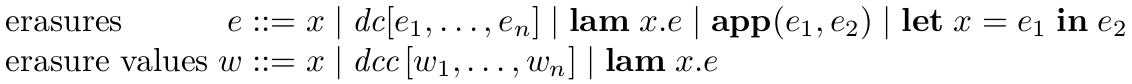
\includegraphics[width=13cm]{img/infig3_erasure.png}
\end{figure}

\noindent すると、動的な項から型消去済の動的な項への変換する、次のような関数 $|\cdot|$ を定義できます。

\begin{figure}[h]
\centering
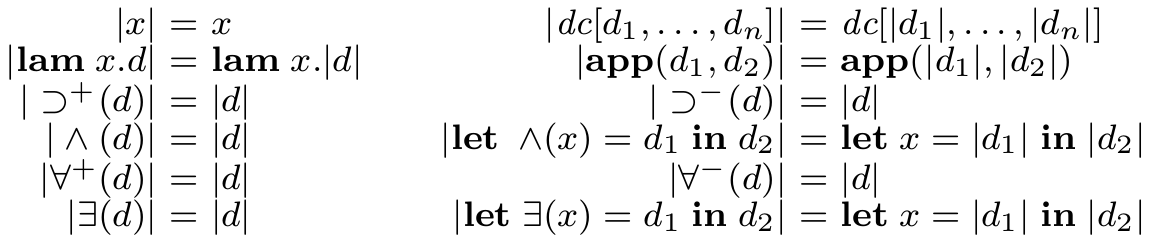
\includegraphics[width=12cm]{img/infig3_trans_erasure.png}
\end{figure}

\noindent {\bf Theorem 3.}
$D :: \emptyset; \emptyset; \emptyset \vdash_S d : s$ を仮定したとき

\begin{enumerate}
  \item もし $d \hookrightarrow^* v$ ならば $|d| \hookrightarrow^* |v|$ です。
  \item もし $|d| \hookrightarrow^* w$ ならば $d \hookrightarrow^* v$ かつ $|v| = w$ であるような値 $v$ が存在します。
\end{enumerate}

\noindent {\it Proof.}
(1) は自明です。(2) は $D$ に対する構造帰納法から得られます。

\noindent Theorem 3 を用いると、型消去済の動的な項 $d$ を単純に評価することで、動的な項 $d$ を評価することができます。

\section{拡張}

この章では、 {\it ATS} を拡張して一般的で現実的なプログラミング機能のいくつかをサポートします。

\noindent {\bf General Recursion}
{\it ATS} で一般帰納 (general recursion) をサポートするために、不動点演算子 {\bf fix} を導入します。
ここでは、変数 $x$ を {\bf lam}変数と呼び、{\bf fix}変数 $f$ を導入します。
 {\bf lam}変数か {\bf fix}変数のいずれかである変数を $xf$ で表わします。

\begin{figure}[h]
\centering
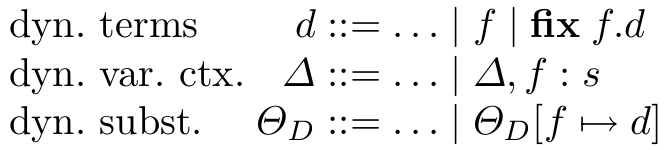
\includegraphics[width=6cm]{img/infig3_general_recursion.png}
\end{figure}

ルール {\bf (ty-var)} が変更を受けるために必要で、ルール {\bf (ty-fix)} に不動点演算子の扱いを追加する必要があります:

\begin{figure}[h]
\centering
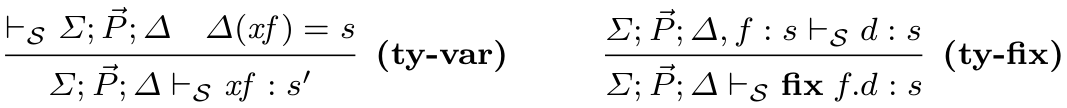
\includegraphics[width=11cm]{img/infig3_fixed-point_op.png}
\end{figure}

\noindent {\bf fix} $f.d$ の動的な項は簡約基で、その簡約は $d[f \mapsto {\bf fix} f.d]$ になります。
この拡張について、subject reduction定理 (Theorem 1) とprogress定理 (Theorem 2) の両方が素直に成立します。

\noindent {\bf Datatypes and Pattern Matching}
{\it ATS} を拡張してデータ型とパターンマッチをサポートするアプローチを示します。
それからいくつかの簡単な例を紹介します。
次のような追加の構文が必要になります。

\begin{figure}[h]
\centering
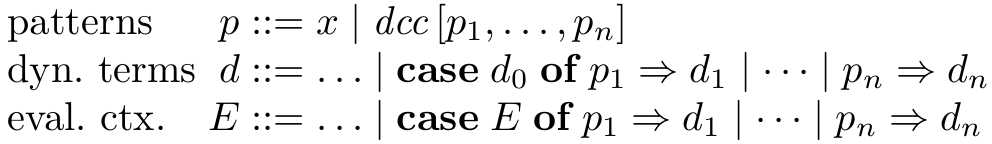
\includegraphics[width=9cm]{img/infig3_pattern_match.png}
\end{figure}

\noindent いつものように、どのような変数 $x$ もパターン中に一度だけ登場できます。
値 $v$ とパターン $p$ が与えられたとき、$v = p[\Theta_D]$ を示すのに $v \Downarrow p \Rightarrow \Theta_D$ の形の判定を使います。
そのような判定を導出するためのルールは次のように与えられます。

\begin{figure}[h]
\centering
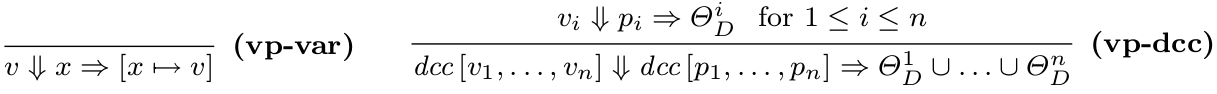
\includegraphics[width=14cm]{img/infig3_vp-doc.png}
\end{figure}

\noindent もし、なんらかの動的な置換 $\Theta_D$ について $v \Downarrow p \Rightarrow \Theta_D$ が導出できるなら、$v$ は $p$ にマッチすると言えます。
ルール {\bf (vp-dcc)} において、$n = 0$ のとき空の動的な置換 $[]$ になるようなユニオン $\Theta^1_D \cup \ldots \cup \Theta^n_D$ は well-defined であることに注意してください。
なぜなら、1つのパターン中にどのような変数も最大一度まで登場できるからです。

$1 \leq i \leq n$ について $v \Downarrow p_i \Rightarrow \Theta_D$ が成立するなら、${\bf case}$ $v$ ${\bf of} p_1 \Rightarrow d_1 |\cdots| p_n \Rightarrow d_n$ の形の動的な項は簡約基で、その簡約は $d_i[\Theta_D]$ になります。
もし $v$ が複数のパターン $p_i$ にマッチするなら、このような簡約基の簡約は非決定論を引き起こすかもしれないことに注意してください。

\begin{figure}[h]
\centering
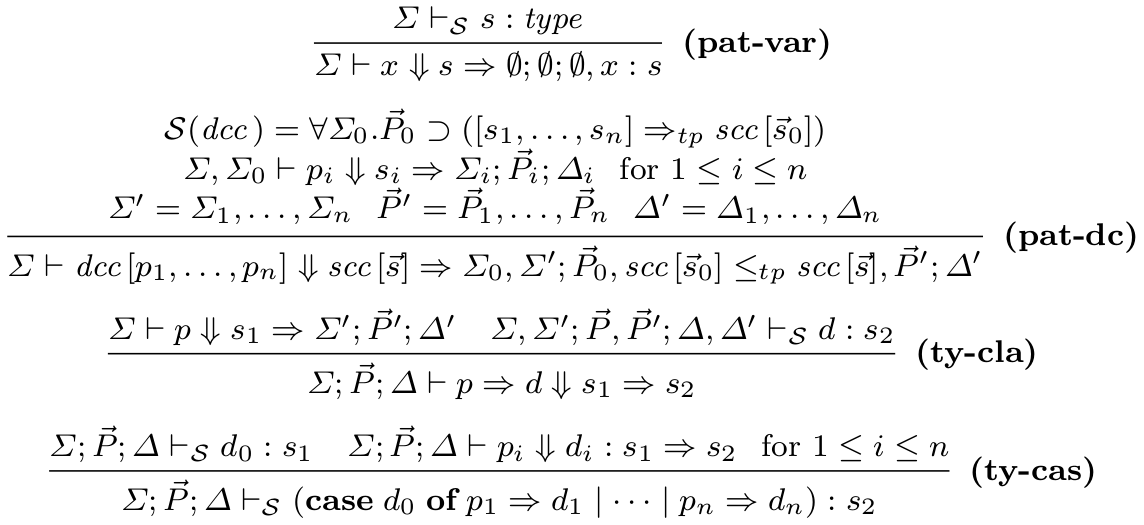
\includegraphics[width=12cm]{img/fig6_rules_pattern_match.png}
\caption{パターンマッチの型付けルール}
\label{fig:fig6_rules_pattern_match}
\end{figure}

パターンマッチの型付けルールを図\ref{fig:fig6_rules_pattern_match} に示します。
$\Sigma \vdash p \Downarrow s \Rightarrow \Sigma'; P'; \Delta'$ の判定の意味は、次の補題で形式的に捕捉されます。

\noindent {\bf Lemma 4.}
$D :: \emptyset;\emptyset;\emptyset \vdash_S v:s, \varepsilon_1::\emptyset \vdash p \Downarrow s \vdash \Sigma; \vec{P}; \Delta$ と $\varepsilon_2 :: v \Downarrow p \Rightarrow \Theta_D$ を仮定します。
すると、$\vec{P}$ のそれぞれの $P$ について $\emptyset;\emptyset \models_S P[\Theta_S]$ であり、かつ $\emptyset;\emptyset;\emptyset \vdash_S \Theta_D : \Delta$ ような $\Theta_S : \Sigma$ が存在します。

\noindent {\it Proof.}
この補題は $\varepsilon_1$ における構造帰納法から得られます。

\noindent 例として、次の判定は導出可能です。

\begin{figure}[h]
\centering
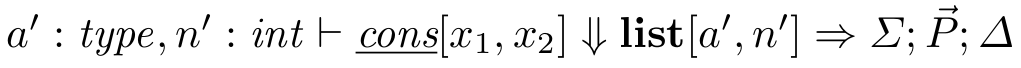
\includegraphics[width=9cm]{img/infig3_lemma4_judgement.png}
\end{figure}

\noindent ここで \underline{$cons$} には次のdc型が割り当てられます。

\begin{figure}[h]
\centering
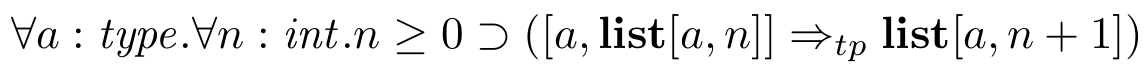
\includegraphics[width=10cm]{img/infig3_lemma4_cons_dctype.png}
\end{figure}

\noindent なおかつ $\Sigma = (a:type, n:int)$、 $\vec{P} = (n \geq 0, {\bf list}[a,n+1] \leq_{tp} {\bf list}[a',n'])$、かつ $\Delta = (x_1:a, x_2:{\bf list}[a,n])$ です。

この拡張においてsubject reduction 定理 (Theorem 1) はすぐに証明できます:
簡約されたインデックスが次の形になる場合を扱うために、Lemma 4が必要になります:

\begin{figure}[h]
\centering
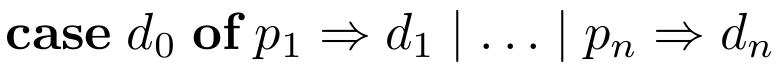
\includegraphics[width=6cm]{img/infig3_lemma4_theorem1.png}
\end{figure}

\noindent また、この拡張においてprogress定理 (Theorem 2) を成立させることができます。
このとき well-typed なプログラム $d$ が次の形を取る可能性を考慮するために、定理のわずかな修正が必要です。

\begin{figure}[h]
\centering
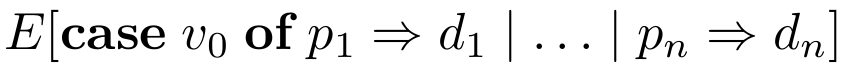
\includegraphics[width=6cm]{img/infig3_lemma4_theorem2.png}
\end{figure}

\noindent ここで、もし $d$ が値でもなく簡約することもできないなら、$1 \leq i \leq n$ について $v_0$ はどのような $p_i$ にもマッチしません。

\noindent {\bf Effects}
{\it PTS} と異なり、{\it ATS} は参照や例外のような作用をサポートする際も素直な方法で拡張できます。
例えば、参照を {\it ATS} に導入するために、sc種 $[type] \Rightarrow type$ の型コンストラクタ $ref$ と、次のように対応するdc型が割り当てられた動的な関数を単純に宣言できます。

\begin{figure}[h]
\centering
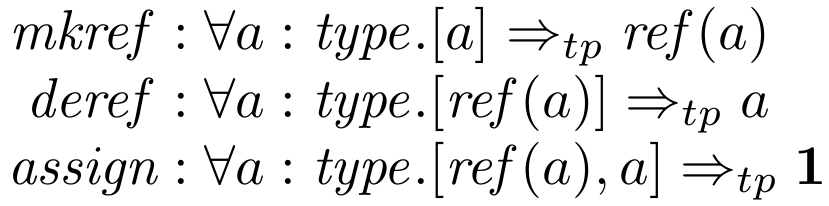
\includegraphics[width=6cm]{img/infig3_effect_dctype.png}
\end{figure}

これらの関数の意図する意味は明らかです。
また、$ref$ が不変の型コンストラクタになってしまう問題に対処するため、Definition 1に次の規則条件を追加する必要があります。

\begin{itemize}
\item $\Sigma; \vec{P} \models_S ref(s) \leq_{tp} ref(s')$ は $\Sigma; \vec{P} \models_S s \leq_{tp} s'$ と $\Sigma; \vec{P} \models_S s' \leq_{tp} s$ を意味します。
\end{itemize}

\noindent この拡張に動的な意味論を割り当てる手法は一般的なもので、subject reduction定理とprogress定理の両方を成立できます。
この手法の詳細については [Har94] を参照してください。

同様に {\it ATS} に例外を導入することも素直な方法で可能です。
そのため詳細は省略します。

\section{Applied Type Systemの例}

驚くことではありませんが、$\lambda$-cube [Bar92] における System $\lambda_2$ と $\lambda_{\omega}$ が applied type system であることは簡単に示すことができます。
また guarded recursive datatypes で $\lambda_2$ を拡張した $\lambda_{G\mu}$ 言語 [XCC03] と Dependent ML [XP99] も applied type system です。
より詳細な説明は [Xi03] を参照してください。

\section{関連研究と結論}

{\it ATS} フレームワークは、依存データ型を使って ML の型システムを改良した Dependent ML [XP99,Xi98] と、最新の研究である guarded recursive datatypes [XCC03] の成果に基づいています。
これら2つの型
\footnote{実際には guarded recursive datatypes を、型が型をインデックスするような "依存型" として考えることができます。}
の間に類似点を見つけた私達は、自然にこれらの統一された表現の探求に導かれました。

Haskellの型クラスの根底にある qualified types [Jon94] に精通した人に対して、qualified type はガード型と見なせないことを指摘しておきます。
その単純な理由は、applied type system におけるガードの証明が計算上の意味を持っていないことです。
つまり、プログラムの実行時の挙動に影響を及ぼすことができないのです。
しかし、qualified types の環境における型の述語の証明である dictionary はプログラムの実行時の挙動に影響を与えることができ、また好んで使われます。

別方向の関連研究として certified binaries [SSTP02] を用いた型システムの形式化があります。
これもまた型とプログラムを完全に分離するアイデアです。
帰納的な定義 (CiC) [PPM89,PM93] を拡張した calculus of constructions にこの型言語は基づいているとはいえ、基本的にこの型システムにおける型言語と計算言語の概念は、それぞれATSのstaticsとdynamicsの概念に相当します。
けれども、ATS における制約関係の概念は [SSTP02] のものに相当するわけではありません。
その代わりに、型の正規形を比較することで、2つの型の等価性を決定できます。
私達が applied type system と関連した制約関係の証明を効果的に表現/検証するアプローチ持っている以上、[SSTP02] の意味での certify binaries に対して applied type system を構築することも困難ではありません。

要約すると、実用的なプログラミングをサポートするための型システムのデザインと形式化を促進するために、{\it ATS} フレームワークを示しました。
statics と dynamics を完全に分離することで、{\it ATS} は作用の存在下における依存型のサポートに特に威力を発揮します。
また、{\it ATS} のガード型とアサート型を使うことで、より柔軟により効果的にプログラムの不変条件を捕捉できます。
これまで研究されてきた依存型 [XP99,Xi98] と guarded recursive datatypes [XCC03] の統一化と一般化であると、 {\it ATS} をとらえることもできます。

現時点では {\it ATS} の静的な要素は単純なラムダ計算に基づいています。
従って、静的な要素が多相性と依存型をサポートする型付きラムダ計算の上に構築できるか研究することができるでしょう。
また、{\it ATS} に基づく型システムを使って関数型プログラミング言語をデザイン/実装することに、私達は特に興味を持っています。
それは既存の言語において新しい言語構造を実装するような方法で、言語拡張を行なう手段を提供できるでしょう。

\begin{acknowledgment}
Assaf Kfouryからこの論文のドラフトに対するコメントをもらいました。
また、Chiyan Chenとはこの論文の主題について議論しました。
感謝します。
\end{acknowledgment}

%\begin{thebibliography}{10}
%\end{thebibliography}

\end{document}
